%===============================================================================
% CHAPTER 15: VAN DEN STEEN DECISION HIERARCHY FRAMEWORK
% Integration of Strategy Theory with Behavioral Change Architecture
%===============================================================================

\documentclass[11pt, a4paper]{article}
\usepackage[utf8]{inputenc}
\usepackage[margin=1in]{geometry}
\usepackage{amsmath, amssymb, amsthm}
\usepackage{booktabs, array, multirow, tabularx}
\usepackage{xcolor}
\usepackage{tcolorbox}
\usepackage{hyperref}
\usepackage{tikz}
\usetikzlibrary{shapes,arrows,positioning,calc}

\title{Chapter 15 Framework: Van den Steen's Theory Applied to Behavioral Intervention Design}
\author{BEATRIX Research Group \\ FehrAdvice \& Partners AG}
\date{January 2026}

\begin{document}

\maketitle

%===============================================================================
\section*{Conceptual Overview: From Strategy to Decision Hierarchies}
%===============================================================================

\begin{tcolorbox}[colback=blue!5!white, colframe=blue!75!black, title=Core Insight]

\textbf{Van den Steen's Theory states:} \textit{Strategy is the smallest set of choices that determines all other choices through complementarity.}

\textbf{Applied to behavioral intervention:} The \textbf{meta-level strategic choice} (e.g., ``Aggressive Transformation'' vs. ``Maintenance'') cascades downward to create \textbf{emergent decision hierarchies}.

\textbf{Critical Recognition:}
\begin{itemize}[nosep]
    \item Number of decision layers is \textbf{NOT fixed} (not always 4)
    \item Layers \textbf{EMERGE} from the strategic choice and context
    \item Aggressive strategies require 2-3$\times$ more coordinated layers than Maintenance
    \item This applies across ALL welfare levels (Individual through Nation)
\end{itemize}

\end{tcolorbox}

%===============================================================================
\section{Decision Layer Emergence: The Complete Matrix}
%===============================================================================

\subsection{Master Table: Layers by Archetype and Welfare Level}

\begin{table}[htbp]
\centering
\caption{Emergent Decision Layers by Meta-Strategic Choice and Welfare Level}
\small
\renewcommand{\arraystretch}{1.4}
\begin{tabularx}{\textwidth}{|l|c|c|c|c|}
\hline
\textbf{Meta-Choice Archetype} & \textbf{Individual (L=0)} & \textbf{Team (L=1)} & \textbf{Org (L=2)} & \textbf{Nation (L=4)} \\
\hline
\cellcolor{red!20}\textbf{Harvesting} (Exit-Oriented) & 1-2 & 2-3 & 2-3 & 3-4 \\
\hline
\cellcolor{yellow!20}\textbf{Maintenance} (Status Quo) & 2-3 & 3-4 & 3-4 & 4-5 \\
\hline
\cellcolor{green!20}\textbf{Balanced} (Incremental) & 3-4 & 4-5 & 4-6 & 6-8 \\
\hline
\cellcolor{blue!20}\textbf{Aggressive} (Transformation) & 4-5 & 5-6 & 6-8 & 8-12+ \\
\hline
\end{tabularx}
\end{table}

\textbf{Interpretation:}
\begin{itemize}[nosep]
    \item Each cell shows the \textit{expected range} of coordinated decision layers
    \item Lower bound: Simple, well-defined context
    \item Upper bound: Complex, multi-stakeholder context
    \item Ranges are \textit{emergent}, not prescriptive
\end{itemize}

%===============================================================================
\section{Decision Layers by Archetype: Detailed Analysis}
%===============================================================================

\subsection{ARCHETYPE 1: HARVESTING (Exit-Oriented)}

\textbf{Meta-Level Definition:} ``Minimize ongoing resources; maximize graceful exit''

\subsubsection{Individual Level: 1-2 Layers}

\begin{tcolorbox}[colback=gray!5!white, colframe=gray!75!black, title=Example: Smoking Cessation via Complete Exit]

\textbf{Scenario:} Individual wants to quit smoking completely, immediately.

\begin{enumerate}
    \item \textbf{Layer 0 (Meta-Choice):} ``Complete cessation'' (no compromise, no harm reduction)

    \item \textbf{Layer 1 (Exit Mechanism):}
    \begin{itemize}[nosep]
        \item Cold turkey vs. gradual taper (likely: cold turkey, derived from meta-choice)
        \item Single quit date vs. flexible? (likely: fixed, reinforces commitment)
        \item Disposal of all tobacco products? (derived from meta-choice)
    \end{itemize}

    \item \textbf{Layer 2 (Optional, if context complex):}
    \begin{itemize}[nosep]
        \item Handling social situations where smoking occurs (avoidance vs. skills)
        \item Contingency plan if relapse occurs
    \end{itemize}
\end{enumerate}

\textbf{Typical Range:} 1-2 layers (high-discipline individuals need 1; socially embedded need 2)

\end{tcolorbox}

\subsubsection{Organization Level: 2-3 Layers}

\begin{tcolorbox}[colback=gray!5!white, colframe=gray!75!black, title=Example: Organizational Spin-off or Divestiture]

\textbf{Scenario:} Company decides to exit a business unit entirely within 18 months.

\begin{enumerate}
    \item \textbf{Layer 0 (Meta-Choice):} ``Complete exit from Product Line X''

    \item \textbf{Layer 1 (Exit Mechanics):}
    \begin{itemize}[nosep]
        \item Sell to competitor vs. liquidate vs. spin-off (derived from exit goal)
        \item Timeline: 6, 12, 18 months? (derived from meta-choice)
        \item Retain which IP/talent? (derived from meta-choice)
    \end{itemize}

    \item \textbf{Layer 2 (Stakeholder Management):}
    \begin{itemize}[nosep]
        \item Employee transition plan (layoffs vs. internal mobility)
        \item Customer communication (wind-down vs. migration)
        \item Supplier obligations (contract unwinding)
    \end{itemize}

    \item \textbf{Layer 3 (Optional):}
    \begin{itemize}[nosep]
        \item Legal/regulatory approvals
        \item Financial restructuring
    \end{itemize}
\end{enumerate}

\textbf{Typical Range:} 2-3 layers (complex corporate exit: 3; simple product discontinuation: 2)

\end{tcolorbox}

---

\subsection{ARCHETYPE 2: MAINTENANCE (Status Quo Preservation)}

\textbf{Meta-Level Definition:} ``Keep current trajectory with minimal change; prevent degradation''

\subsubsection{Individual Level: 2-3 Layers}

\begin{tcolorbox}[colback=gray!5!white, colframe=gray!75!black, title=Example: Habit Reinforcement (e.g., Regular Exercise)]

\textbf{Scenario:} Individual currently exercises 3x/week; goal is to sustain without regression.

\begin{enumerate}
    \item \textbf{Layer 0 (Meta-Choice):} ``Maintain current activity level (3x/week exercise)''

    \item \textbf{Layer 1 (Sustainability Mechanisms):}
    \begin{itemize}[nosep]
        \item Environmental cue structure (where/when to exercise)
        \item Social commitment device (workout buddy vs. solo)
        \item Default incentives (gym membership auto-renews?)
    \end{itemize}

    \item \textbf{Layer 2 (Contingency Planning):}
    \begin{itemize}[nosep]
        \item How to respond if missing one session (automatic re-scheduling?)
        \item What triggers intervention to prevent relapse?
        \item Who monitors adherence?
    \end{itemize}
\end{enumerate}

\textbf{Typical Range:} 2-3 layers (simple routine: 2; socially embedded: 3)

\end{tcolorbox}

\subsubsection{Organization Level: 3-4 Layers}

\begin{tcolorbox}[colback=gray!5!white, colframe=gray!75!black, title=Example: Organizational Steady State (e.g., Market Share Maintenance)]

\textbf{Scenario:} Company currently holds 25\% market share; goal is to maintain (not lose ground).

\begin{enumerate}
    \item \textbf{Layer 0 (Meta-Choice):} ``Defend current market position; no expansion''

    \item \textbf{Layer 1 (Core Business Levers):}
    \begin{itemize}[nosep]
        \item Price maintenance strategy (stable vs. competitive defense)
        \item Quality assurance level (maintain current, no R\&D investment)
        \item Distribution channels (keep current, no new channels)
    \end{itemize}

    \item \textbf{Layer 2 (Threat Response):}
    \begin{itemize}[nosep]
        \item Customer retention program (loyalty incentives)
        \item Competitive monitoring (early warning system)
        \item Cost management (to offset any margin pressure)
    \end{itemize}

    \item \textbf{Layer 3 (Organizational Calibration):}
    \begin{itemize}[nosep]
        \item Staffing levels (stable headcount)
        \item Capital expenditure (maintenance capex only)
        \item Organizational structure (no major reorganization)
    \end{itemize}
\end{enumerate}

\textbf{Typical Range:} 3-4 layers (simple market: 3; complex competitor landscape: 4)

\end{tcolorbox}

---

\subsection{ARCHETYPE 3: BALANCED GROWTH (Incremental Improvement)}

\textbf{Meta-Level Definition:} ``Grow steadily; balance ambition with stability; accept some disruption''

\subsubsection{Individual Level: 3-4 Layers}

\begin{tcolorbox}[colback=gray!5!white, colframe=gray!75!black, title=Example: Career Development (e.g., Skill Enhancement)]

\textbf{Scenario:} Individual works full-time; wants to gain new professional skills while maintaining employment.

\begin{enumerate}
    \item \textbf{Layer 0 (Meta-Choice):} ``Acquire new skills in 12-18 months while maintaining current role''

    \item \textbf{Layer 1 (Learning Architecture):}
    \begin{itemize}[nosep]
        \item Which skills? (language vs. technical vs. leadership)
        \item Learning mode (coursework vs. mentorship vs. project-based)
        \item Time commitment (5 hrs/week vs. 10 hrs/week)
    \end{itemize}

    \item \textbf{Layer 2 (Integration Strategy):}
    \begin{itemize}[nosep]
        \item How to apply new skills in current role? (project volunteering)
        \item Communication to manager (transparency vs. strategic silence)
        \item Internal network cultivation (mentors, peers)
    \end{itemize}

    \item \textbf{Layer 3 (Transition Planning):}
    \begin{itemize}[nosep]
        \item Career move timing (after certification? after visible results?)
        \item Target roles with new skills
        \item Contingency if market conditions shift
    \end{itemize}
\end{enumerate}

\textbf{Typical Range:} 3-4 layers (focused single skill: 3; multi-domain development: 4)

\end{tcolorbox}

\subsubsection{Organization Level: 4-6 Layers}

\begin{tcolorbox}[colback=gray!5!white, colframe=gray!75!black, title=Example: Digital Modernization (Incremental Implementation)]

\textbf{Scenario:} Manufacturing company modernizes IT systems while maintaining production; targets 15-20\% productivity gain over 3 years.

\begin{enumerate}
    \item \textbf{Layer 0 (Meta-Choice):} ``Implement modern tech stack; phased approach; zero production downtime''

    \item \textbf{Layer 1 (Technology Strategy):}
    \begin{itemize}[nosep]
        \item Which systems first? (ERP, CRM, supply chain, etc.; sequencing matters)
        \item Cloud vs. on-premise? (likely: hybrid, to limit disruption)
        \item Build vs. buy vs. customize? (likely: buy, minimizes disruption)
    \end{itemize}

    \item \textbf{Layer 2 (Implementation Approach):}
    \begin{itemize}[nosep]
        \item Pilot vs. phased rollout (pilot in non-critical dept first)
        \item Change management intensity (training scope, communication cadence)
        \item Parallel-running period (old + new systems running together? For how long?)
    \end{itemize}

    \item \textbf{Layer 3 (Skill Development):}
    \begin{itemize}[nosep]
        \item Who learns the new systems? (power users vs. all staff)
        \item Training timing relative to implementation (before, during, after?)
        \item Knowledge transfer from vendor (train-the-trainer model?)
    \end{itemize}

    \item \textbf{Layer 4 (Governance \& Decision Rights):}
    \begin{itemize}[nosep]
        \item Who makes go/no-go decisions at each phase?
        \item Escalation path if issues arise?
        \item Success criteria to move to next phase?
    \end{itemize}

    \item \textbf{Layer 5 (Risk Mitigation):}
    \begin{itemize}[nosep]
        \item Contingency plan if productivity drops? (roll-back procedures)
        \item Customer communication if service is impacted?
        \item Financial buffer for unexpected costs?
    \end{itemize}
\end{enumerate}

\textbf{Typical Range:} 4-6 layers (simple, contained modernization: 4; complex, multi-system: 6)

\end{tcolorbox}

---

\subsection{ARCHETYPE 4: AGGRESSIVE TRANSFORMATION}

\textbf{Meta-Level Definition:} ``Fundamental change; accept high disruption for transformation; new business model / mindset''

\subsubsection{Individual Level: 4-5 Layers}

\begin{tcolorbox}[colback=gray!5!white, colframe=gray!75!black, title=Example: Major Life Transition (e.g., Career Pivot to New Field)]

\textbf{Scenario:} Individual in mid-career (age 35) completely changes fields (e.g., law to data science); expects 1-2 year transition.

\begin{enumerate}
    \item \textbf{Layer 0 (Meta-Choice):} ``Complete career transformation; accept income loss and status drop; commit to new identity''

    \item \textbf{Layer 1 (Skill Acquisition):}
    \begin{itemize}[nosep]
        \item Intensive bootcamp vs. gradual degree? (likely: intensive bootcamp, signals commitment)
        \item Location change? (move to tech hub?)
        \item Full-time study vs. part-time? (likely: full-time, to enable faster transformation)
    \end{itemize}

    \item \textbf{Layer 2 (Identity \& Belief Alignment):}
    \begin{itemize}[nosep]
        \item How to internalize new identity (e.g., ``I am a data scientist'')?
        \item Social circle shift (who validates the new identity?)
        \item Family alignment (partner, parents understanding the change?)
    \end{itemize}

    \item \textbf{Layer 3 (Financial Architecture):}
    \begin{itemize}[nosep]
        \item Income sources during transition (savings? Partner income? Loan?)
        \item Timeline to job market readiness (months to employment target?)
        \item Expected income trajectory (how long to recover pre-transition earnings?)
    \end{itemize}

    \item \textbf{Layer 4 (Contingency \& Adaptation):}
    \begin{itemize}[nosep]
        \item What triggers going back? (if unable to find job after X months?)
        \item Partial path (hybrid roles that bridge old/new?)
        \item Ongoing support structure (mentors in new field?)
    \end{itemize}
\end{enumerate}

\textbf{Typical Range:} 4-5 layers (supported transition: 4; unsupported with family resistance: 5)

\end{tcolorbox}

\subsubsection{Organization Level: 6-8 Layers}

\begin{tcolorbox}[colback=gray!5!white, colframe=gray!75!black, title=Example: Business Model Transformation (e.g., Hardware to Software-as-a-Service)]

\textbf{Scenario:} Legacy manufacturing company transforms to SaaS model; 2-3 year transformation; involves new revenue model, organization, culture.

\begin{enumerate}
    \item \textbf{Layer 0 (Meta-Choice):} ``Transform from product sales to subscription revenue; accept initial revenue decline; build recurring revenue model''

    \item \textbf{Layer 1 (Business Model Architecture):}
    \begin{itemize}[nosep]
        \item Pricing model (seat-based? Usage-based? Value-based?)
        \item Go-to-market (direct sales? Self-serve? Hybrid?)
        \item Customer success requirements (proactive support vs. reactive?)
    \end{itemize}

    \item \textbf{Layer 2 (Product Architecture):}
    \begin{itemize}[nosep]
        \item Cloud hosting (build internal? AWS? Multi-cloud?)
        \item Modularity (monolithic vs. microservices? This affects scalability)
        \item Integration requirements (API-first vs. standalone?)
    \end{itemize}

    \item \textbf{Layer 3 (Organizational Restructuring):}
    \begin{itemize}[nosep]
        \item Organizational chart (new functional divisions for SaaS?)
        \item Reporting lines (product, engineering, customer success structure?)
        \item Skill requirements (hire data scientists? Customer success managers?)
    \end{itemize}

    \item \textbf{Layer 4 (Revenue \& Financial Model):}
    \begin{itemize}[nosep]
        \item Pricing tier structure (starter, pro, enterprise?)
        \item Revenue recognition (ASP targets? Churn tolerances?)
        \item Financial KPIs (CAC, LTV, gross margin targets?)
    \end{itemize}

    \item \textbf{Layer 5 (Culture \& Capability Building):}
    \begin{itemize}[nosep]
        \item Mindset shift from ``ships product once'' to ``continuous updates''
        \item Employee training (new roles, new metrics, new skills)
        \item Leadership alignment (old guard product mindset vs. new SaaS mindset)
    \end{itemize}

    \item \textbf{Layer 6 (Market \& Competitive Strategy):}
    \begin{itemize}[nosep]
        \item Competitive positioning (vs. cloud-native SaaS startups)
        \item Customer acquisition channels (leverage installed base? Or go new market?)
        \item Win-back vs. new customer strategy
    \end{itemize}

    \item \textbf{Layer 7 (Transition Mechanics):}
    \begin{itemize}[nosep]
        \item Parallel business model (maintain old product while building SaaS?)
        \item Customer migration strategy (force upgrades? Incentivize? Slow wind-down?)
        \item Go-no-go decision points (when to sunset old product?)
    \end{itemize}
\end{enumerate}

\textbf{Typical Range:} 6-8 layers (focused single product: 6; multiple product lines, multiple geographies: 8)

\end{tcolorbox}

\subsubsection{Nation Level: 8-12+ Layers}

\begin{tcolorbox}[colback=gray!5!white, colframe=gray!75!black, title=Example: National Climate Neutrality (e.g., Carbon Reduction Transformation)]

\textbf{Scenario:} Nation commits to carbon neutrality by 2040 (14 years from 2026); involves energy, transport, industry, agriculture.

\begin{enumerate}
    \item \textbf{Layer 0 (Meta-Choice):} ``Carbon neutral by 2040; technology-driven, economically sustainable, no energy poverty''

    \item \textbf{Layer 1 (Energy Architecture):}
    \begin{itemize}[nosep]
        \item Renewable mix (wind, solar, hydro, nuclear? What \%?)
        \item Grid transformation (decentralized vs. centralized?)
        \item Storage requirements (batteries, pumped hydro, hydrogen?)
    \end{itemize}

    \item \textbf{Layer 2 (Transport Transition):}
    \begin{itemize}[nosep]
        \item EV adoption targets and timeline
        \item Public transit expansion requirements
        \item Aviation/shipping decarbonization pathways
    \end{itemize}

    \item \textbf{Layer 3 (Industrial Transformation):}
    \begin{itemize}[nosep]
        \item Heavy industry decarbonization (cement, steel, chemicals)
        \item Circular economy requirements
        \item Export competitiveness concerns
    \end{itemize}

    \item \textbf{Layer 4 (Agriculture \& Land Use):}
    \begin{itemize}[nosep]
        \item Methane reduction from livestock
        \item Forestry and carbon sequestration targets
        \item Food system transformation
    \end{itemize}

    \item \textbf{Layer 5 (Workforce Transition):}
    \begin{itemize}[nosep]
        \item Reskilling programs for fossil fuel workers
        \item New job creation in green sectors
        \item Regional economic diversification
    \end{itemize}

    \item \textbf{Layer 6 (Investment \& Financing):}
    \begin{itemize}[nosep]
        \item Public sector funding requirements
        \item Private sector incentives (tax credits, subsidies?)
        \item International climate finance mechanisms
    \end{itemize}

    \item \textbf{Layer 7 (Governance \& Coordination):}
    \begin{itemize}[nosep]
        \item Federal/local coordination mechanisms
        \item Regulatory framework updates
        \item International commitments and verification
    \end{itemize}

    \item \textbf{Layer 8 (Behavioral \& Social Change):}
    \begin{itemize}[nosep]
        \item Consumer behavior change (reduced consumption? Different patterns?)
        \item Social license (public acceptance of changes?)
        \item Narrative/identity shift (``green'' identity adoption)
    \end{itemize}

    \item \textbf{Layer 9 (Just Transition Mechanisms):}
    \begin{itemize}[nosep]
        \item Support for affected communities
        \item Intergenerational equity
        \item Distributional impacts management
    \end{itemize}

    \item \textbf{Layer 10 (International Coordination):}
    \begin{itemize}[nosep]
        \item Trade implications (carbon border adjustments?)
        \item Technology transfer to developing nations
        \item Competitive dynamics with other countries
    \end{itemize}
\end{enumerate}

\textbf{Typical Range:} 8-12+ layers (simple economy with few sectors: 8; complex, wealthy, diverse: 12+)

\end{tcolorbox}

---

%===============================================================================
\section{Understanding Layer Emergence: Why These Numbers?}
%===============================================================================

\subsection{Complementarity Creates Layers}

Each decision layer represents a set of \textbf{interdependent choices} that must be coordinated because they are complements.

\textbf{Example: SaaS Transformation (Layer 1 + Layer 2 interdependence):}

\begin{itemize}
    \item If Layer 1 chooses: ``Freemium model with self-serve onboarding''
    \item Then Layer 2 is CONSTRAINED: Must choose ``cloud-native, fully automated infrastructure''
    \item If Layer 2 chose: ``Legacy on-premise infrastructure,'' it would be INCOHERENT with Layer 1
    \item Incoherence = efficiency loss (Appendix BB)
\end{itemize}

\subsection{Ambition Drives Layer Count}

Why does Aggressive have 2-3$\times$ more layers than Maintenance?

\begin{enumerate}
    \item \textbf{Scope of change:} Aggressive touches more domains (individuals, teams, culture, incentives, governance)
    \item \textbf{Coordination complexity:} Each domain needs its own decisions + alignment with others
    \item \textbf{Contingency planning:} More ambitious changes require more ``if-then'' scenarios
    \item \textbf{Identity/belief alignment:} Transformation requires stakeholders to internalize new identities; maintenance doesn't
\end{enumerate}

\subsection{Context Complexity Drives Layer Count}

Why does Nation level have 8-12+ layers while Individual has 4-5?

\begin{enumerate}
    \item \textbf{Number of subsystems:} Individual has 1; Nation has many (energy, transport, industry, agriculture, etc.)
    \item \textbf{Stakeholder heterogeneity:} Individual is mostly one; Nation involves millions with conflicting interests
    \item \textbf{Governance levels:} Individual: self; Organization: ~5 levels; Nation: 3+ (local, regional, national)
    \item \textbf{Implementation lags:} Nation-level infrastructure takes years; individual weeks/months
\end{enumerate}

%===============================================================================
\section{Practitioner Decision Protocol}
%===============================================================================

\subsection{How to Determine Your Intervention Layers}

\textbf{Step 1: Clarify the Meta-Choice}

Write down your strategic commitment in one sentence:

\begin{center}
\framebox[1.2\width]{\begin{minipage}{0.9\textwidth}
    ``We commit to [SPECIFIC OUTCOME] by [DATE] at [WELFARE LEVEL], accepting [TRADE-OFFS].''

    Examples:
    \begin{itemize}[nosep]
        \item Individual: ``Complete smoking cessation within 6 months''
        \item Organization: ``50\% reduction in plastic packaging by 2028''
        \item Nation: ``Carbon neutrality by 2040''
    \end{itemize}
\end{minipage}}
\end{center}

\textbf{Step 2: Identify Your Archetype}

Ask yourself: ``On a scale from Harvesting to Aggressive, where are we?''

\begin{center}
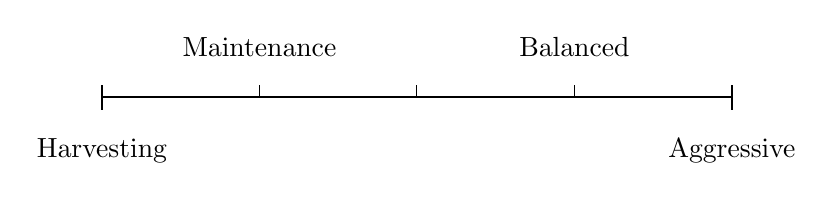
\begin{tikzpicture}[scale=0.8]
    \draw[thick] (0,0) -- (10,0);
    \draw[thick] (0,-0.2) -- (0,0.2);
    \draw[thick] (10,-0.2) -- (10,0.2);
    \node[below] at (0,-0.5) {Harvesting};
    \node[below] at (10,-0.5) {Aggressive};
    \node[above] at (2.5,0.5) {Maintenance};
    \node[above] at (7.5,0.5) {Balanced};
    \draw (2.5,0) -- (2.5,0.2);
    \draw (5,0) -- (5,0.2);
    \draw (7.5,0) -- (7.5,0.2);
\end{tikzpicture}
\end{center}

\textbf{Step 3: Look up Expected Layer Count}

From Table 1, find the range for your archetype + welfare level.

\begin{center}
\textit{Example: Organizational SaaS transformation (Aggressive, Organization) = 6-8 layers}
\end{center}

\textbf{Step 4: Enumerate Your Layers}

Work through Sections 2-5 and identify which layer numbers apply to your context.

\begin{center}
\textit{Example (continued):}
\begin{itemize}[nosep]
    \item Layer 0: Business model architecture (recurring revenue)
    \item Layer 1: Product/tech architecture
    \item Layer 2: Organizational restructuring
    \item Layer 3: Revenue \& financial model
    \item Layer 4: Culture \& capability
    \item Layer 5: Market \& competitive strategy
    \item Layer 6: Transition mechanics
\end{itemize}
\end{center}

\textbf{Step 5: Check Coherence}

For each layer, ask: ``Is this choice coherent with the meta-choice?''

If NO → Revise the choice or reconsider the meta-choice.

%===============================================================================
\section{Connection to Previous Frameworks}
%===============================================================================

\subsection{Integration with Appendix BB (Equilibrium Diagnostics)}

\begin{table}[htbp]
\centering
\caption{How Van den Steen + BB Create a Complete Framework}
\begin{tabular}{|l|p{6cm}|}
\hline
\textbf{Framework} & \textbf{Contributes} \\
\hline
Appendix BB & Diagnostic ($\xi$, $\kappa_{crit}$), drift rates, optimal intervention intensity \\
\hline
Van den Steen & Strategy definition, layer emergence, coherence requirements \\
\hline
Appendix AV & Willingness modeling at each layer (W11-W13) \\
\hline
Appendix B & Complementarity theory (why layers must coordinate) \\
\hline
\end{tabular}
\end{table}

\textbf{Workflow:}
\begin{enumerate}
    \item \textbf{Diagnose (BB):} What is the current equilibrium? How bad is drift?
    \item \textbf{Strategy (VdS):} What meta-choice are we making?
    \item \textbf{Design (VdS + Layers):} How many layers must be coordinated?
    \item \textbf{Operationalize (AV):} How do we ensure willingness at each layer?
    \item \textbf{Execute (Implementation):} Roll out in a way that maintains coherence
\end{enumerate}

%===============================================================================
\section{Open Questions for Chapter 15 Development}
%===============================================================================

\begin{enumerate}
    \item \textbf{Quantifying layer count:} Can we develop a formula relating context complexity to expected layers?

    \item \textbf{Layer interdependence:} How tightly must layers be coupled? Can some decisions proceed in parallel?

    \item \textbf{Adaptive layering:} Can layer structure change during implementation? What triggers changes?

    \item \textbf{Cross-welfare coherence:} When Nation-level strategy conflicts with Individual-level choice, how do we manage?

    \item \textbf{Failure modes:} What happens if layers are misaligned? Can we predict efficiency losses?
\end{enumerate}

%===============================================================================
\end{document}
